\documentclass[10pt,twocolumn]{article}
\usepackage[margin=0.8in]{geometry}
\usepackage{graphicx}
\usepackage{caption}
\usepackage{hyperref}
\usepackage{titlesec}
\usepackage{titling}

% ✅ 中文支持
\usepackage{luatexja}
\usepackage{luatexja-fontspec}

% ✅ 设置中文字体
\setmainjfont{WenQuanYi Zen Hei}

\setlength{\droptitle}{-3em}
\setlength{\parskip}{0pt}

\titlespacing{\section}{0pt}{0.8em}{0.4em}
\titlespacing{\subsection}{0pt}{0.6em}{0.3em}

\pretitle{\vspace{-3em} \begin{center}\LARGE\bfseries}
\posttitle{\end{center}\vspace{-1.2em}}
\preauthor{\begin{center}\normalsize}
\postauthor{\end{center}\vspace{-1.5em}}

% 标题和作者信息
\title{\textbf{Multimodal Stock Price Prediction: A Case Study of the Russian Securities Market}}
\author{
    Kasymkhan Khubiyev, Mikhail Semenov\\
    Sirius University of Science and Technology, Sirius, Russia
}

\begin{document}
\maketitle

\noindent \textbf{摘要:} 本文提出了一种结合蜡烛图时间序列和文本新闻流数据的多模态方法,用于预测金融资产价格。实验结果表明,加入文本模态后,预测的平均绝对百分比误差(MAPE)降低了55\%。

\vspace{0.5em}

\section{引言}
构建资产价格预测是金融市场参与者的重要任务,能够实现战略规划、投资组合管理和风险评估。随着深度学习模型的普及,研究者们开始关注神经网络的应用。同时,新闻流作为影响市场行为的关键因素,其准确性问题随着生成式人工智能模型和大型语言模型(LLMs)的快速发展而被重新审视。本文旨在展示一种新的多模态方法的优势,并提出一个俄语金融新闻数据集。

\section{方法}
本文提出了一种新的多模态方法,将新闻流整合到时间序列数值数据中。新闻文本被转换为向量表示,并与时间序列向量一起输入模型。我们使用预训练模型RuBERT和Vikhr-Qwen2.5-0.5b-Instruct处理文本数据,使用LSTM递归神经网络处理时间序列和向量化文本数据。

\begin{figure}[h]
    \centering
    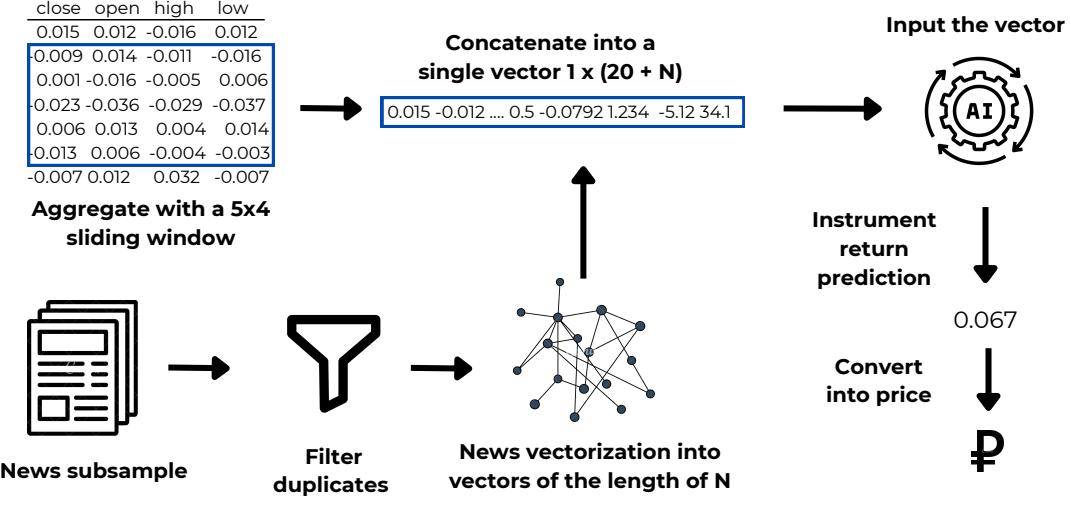
\includegraphics[width=0.9\linewidth]{_page_6_Figure_2.jpeg}
    \caption{资产的归一化收盘价。市场阶段转换日期由垂直虚线表示。}
\end{figure}

\section{实验设计}
我们收集了一个包含176只在莫斯科交易所交易的俄罗斯股票的时间序列数据和79,555篇俄语金融新闻文章的独特数据集。实验分为两部分:仅使用时间序列数据的单模态方法和结合新闻流数据的多模态方法。预测质量通过两个关键指标评估:准确率(Accuracy)和平均绝对百分比误差(MAPE)。

\section{实验结果与分析}
实验结果表明,加入文本模态后,预测的平均绝对百分比误差(MAPE)降低了55\%。表1和表2分别展示了单模态和多模态方法的预测质量指标。

\begin{table}[h]
\centering
\caption{单模态方法预测结果}
\begin{tabular}{lcc}
\hline
模型 & 准确率 & MAPE \\
\hline
LSTM & 52.020\% & 0.397 \\
XGB & 45.000\% & 1.627 \\
KNN & 46.010\% & 1.631 \\
RF & 48.384\% & 1.646 \\
LinReg & 50.152\% & 1.669 \\
DT & 49.798\% & 1.824 \\
\hline
\end{tabular}
\end{table}

\begin{table}[h]
\centering
\caption{多模态方法预测结果}
\begin{tabular}{lcc}
\hline
模型 & 准确率 & MAPE \\
\hline
LSTM-Qwen-Mean & 48.552\% & 0.256 \\
LSTM-Qwen-Sum & 46.970\% & 0.367 \\
LSTM & 52.020\% & 0.397 \\
LSTM-RuBert-Mean & 49.798\% & 0.437 \\
LSTM-RuBert-Sum & 48.148\% & 0.445 \\
\hline
\end{tabular}
\end{table}

\section{结论}
本文提出了一种新的多模态方法,将新闻流整合到时间序列数值数据中,显著提高了资产价格预测的准确性。未来的研究方向包括优化文本模态参数,如时间窗口、情感和新闻消息的时间顺序。

\end{document}